\chapter{The Block Controller Node Hardware}

So far, we covered a lot of ground. The Layout Control System rests on the concept of a node with ports and a common bus for nodes to communicate with each other. There are specialized nodes, one of them being the base station responsible for managing the locomotive sessions and generating the DCC signals. The base station is as the name suggest a central piece in a layout. The base station node shown in the previous chapter featured two track outputs, MAIN and PROG. The MAIN track is what powers the layout. However, the base station power module unit allowed for about 2.5 Amps and hence only smaller layouts will just do fine with one base station. For larger layouts, help to power several track sections is needed.

A common approach is to divide the layout in several sections or blocks and power them individually with a booster or block controller. Such a booster or block controller would be very similar to a base station in that it provides control about the track, current consumption limits and so on. In contrast to a base station a booster or block controller would not produce its own DCC signal or manage a locomotive session but rather use the signal distributed via the LCS bus. Being an LCS node, the block controller will offer a rich set of attributes to manage and query the state and configuration. Again, wherever the functionality is the same that can be found on the base station, there will be the same attributes and functions.

But there is more to it. For a safe and automated operation, dividing the layout on to track blocks with block sections, and block signaling concepts are necessary. A train movement is always a planned movement and hence the track route needed for the movement is authorized from a central operations place. The chapter on block signaling control provided a high level overview on the block signaling concepts. This chapter will provide a big step into automating a layout by introducing the block controller.

Conceptually, a booster and a block controller have very much in common. They both handle a section or block, they both need power modules to generate the track power, they both need to offer basic sensor and control capabilities to manage a track section or block. Our concept will just unify these two modules types and we will call them block controller from now on. A block controller is a LCS node that manages a track. There are versions with one channel, i.e. one block, and two channels. Support for track occupancy detection, an essential feature for block control, is optional since simple boosters would not need it if they just manage one block with no sections. The text will just use the term block controller and only mention boosters explicitly when needed. Let's get started with the overall requirements.

\section{Requirements}

Traditionally, block control in a layout system was implemented with central control electronics and/or relays. This introduced not only a significant amount of cabling but also a high complexity in building a block control system. A centralized place for all the parts of a block system also results in long cable connections running in parallel which act like antennas resulting in face signals. As a general rule, cable connections on a model railroad should be as short as possible. With a decentralized concept where each block or a small number of blocks are managed by a dedicated controller, the lines to tracks, detectors and signals can be much shorter. There may be still a central base station, but the cables to track, switches and signals are just connected to local booster units located next to them. Over the years, the rise of digital control helped to simplify the configuration and building but the central approach still dominates most designs along with the high cabling effort. A digital system, for example, will still need the track occupancy network, perhaps RailCom detectors and a network of boosters to control the layout sections.

As discussed before a large part of the hardware building blocks to run analog and digital equipment in a block system are identical. Both need the same track sections with occupancy detectors and a H-bride as a power module. All the rest can be done in software. If the engine-ID indicate an analog engine the H-bridge will power the track via PWM signals, in case of a digital engine the H-bridge power the track with DCC signals. So, running trains with analog and digital behind each other is just a question of software and without need for additional hardware. You just can’t mix analog and digital on the same block.

A layout is divided into blocks and each block has several sections. For each block and each section in that block a way needs to be found to feed either analog PWM style signals or digital DDC or other protocol based signals along with the safety mechanisms for engines of either type moving from block to block. A key requirement for our block controller is to accommodate this mixed mode running engines. A block is the unit of control on a layout with block signaling. For configuration purposes it has a unique ID, the block Id. Since a layout is fixed once built, the linkages between blocks is too. A block has as the most important attribute the block entry speed. For example, a block occupied has an entry speed of zero. That is an engine following needs to stop at the signal guarding the entry to the occupied block. Block speed can of course vary. For a free block it is the configured maximum block speed, for an occupied block it is zero, and otherwise anything in between depending on the state of the following block and the type and speed of the train.

Blocks can be entered from only one or both directions. While this requirement does not change the basic mechanism of block section occupancy detection, it will change the algorithms implemented. The block algorithm for bi-directional mode routes needs to put at least two stop blocks ahead of them between two trains entering a route to avoid a head on collision. Still, for a bidirectional line, the route direction needs to be set to avoid two trains entering that route in the first place. Our controller needs to be able to be part of a route configuration process. When talking about routes the key requirements is that each block and possible a turnout in the block can be managed centrally from a control panel. All blocks need to offer stair state on demand. The signals along the route are entirely controlled by the state, i.e entry speed, of the block.They are just indicators. Modern block signaling systems do not even have signals, but most model railroader will have signals just to make the layout more interesting. But imagine a staging yard where the block control algorithms will still be there but no signals are there.

Both analog and digital block modes need a way to know where the train actually is within the block and a way to manage the speed change. For example, when the next block is having an entry speed of zero, the train needs to be decelerated to that speed, i.e. it needs to halt at the end of the block. Whether analog or digital, it will translate to either sending digital commands to the engine, or to reducing the track voltage for analog systems. A key requirement is therefore either knowing exactly where the train is within the block or having a way to measure the actual speed to change it accordingly. This topic is explained further in the firmware section of this chapter.

Blocks can have an optional turnout on the entry and the exit. In other words, there are up to two entries to a block and up to two exits. This basic element forms the building block for a layout. The actual setting of the turnout and track occupancy influences the route checking and need also to be broadcasted to all interested parties. The requirement is that the neighbor blocks and as well as any control panel need to receive these events and act accordingly. During power up or restart after a power failure, the setting of the turnout need to be recreated. The requirement is either that the actual setting can be queried or that the last setting is stored in a non-volatile memory so that after a restart the turnout can just be set. However, the safest way is to have sensors for detecting the actual turnout setting.

For digital operations, there is also the requirement for supporting RailCom. A block controller extension should have the optional capability to include a RailCom detector. This detector is also used to identify the actual engine occupying the block. For analog operations the block controller can only detect that there is an engine. Other ways of identifying the engine are needed. It is not a key requirement per se that analog and digital operations are possible simultaneously. But as described in the analog operations chapter there are good reasons to support both modes in one layout. If implemented, the overall layout control needs to manage the type of engine occupying a block and ensure that the next block to enter has the same mode. More on this in the firmware section of this chapter.

\section{Overall hardware module design}

For the design of the hardware module, there are two basic ways. As said, one way is to implement a central approach to the management of all the blocks, the other is a decentralized approach where each block is managed separately. Our block control system implements the latter. It is a decentralized system where a block controller manages two, perhaps four blocks. There is no real limit, but the more blocks are managed by one block controller, the more cabling is required, up to having one block controller managing all blocks, and thus we are back to a central approach. The requirements for a decentralized approach are that all components required to manage a block are bundled in the block controller and perhaps extension board.

Each \textbf{block controller board} will have a main controller based board with the power module circuitry and RailCom detectors. This board alone will also cover all features needed for a booster node. In addition, the\textbf{ block controller extension board} will cover the needs for occupancy detection, turnout and signal control. Depending on the hardware types, there are different turnouts and signal drivers. Again, we could design a separate extension board for the track occupancy and another one for the turnout and signal control. Both can be connected to the block controller main board.

While all this may sound like a hardware overkill, the occupancy detectors the turnout and signals drivers need to be in place anyhow. So are the boosters. There are only the number of power modules, one per block, instead of few boosters along the layout required. But having a power module for each bock gives us a good way to manage analog and digital blocks in one layout. And the prices for a H-Bridge chip that controls two blocks is quite reasonable so far.

The next sections present two block controller boards, a quad block controller and a dual block controller board. While not every layout will favor a quad block controller, scaling the design down to two or even one block is rather straightforward. The dual block controller offers two blocks or one block with a higher amperage. We will start with the quad block controller, since the dual block controller is just a scaled down version of the building blocks used.

\section{Quad Block Controller}

\subsection{Block Diagram}

The following schematics show the block controller board for the quad block version. First, there is the main controller part with the connectors, the Raspberry PI PICO, the non-volatile memory, the CAN Bus line driver and the level shifters for the external connector pins used. Note that all the digital pins DIO0 to DIO7 are not exported, they are used on the board itself. The block controller also make use of the track lane connector, which routes the track power signals from the block controller board to the extension board. This way, no extra cables need to be wired from block controller to extension board for this purpose. 

\begin{figure}[htbp]
    \centering
    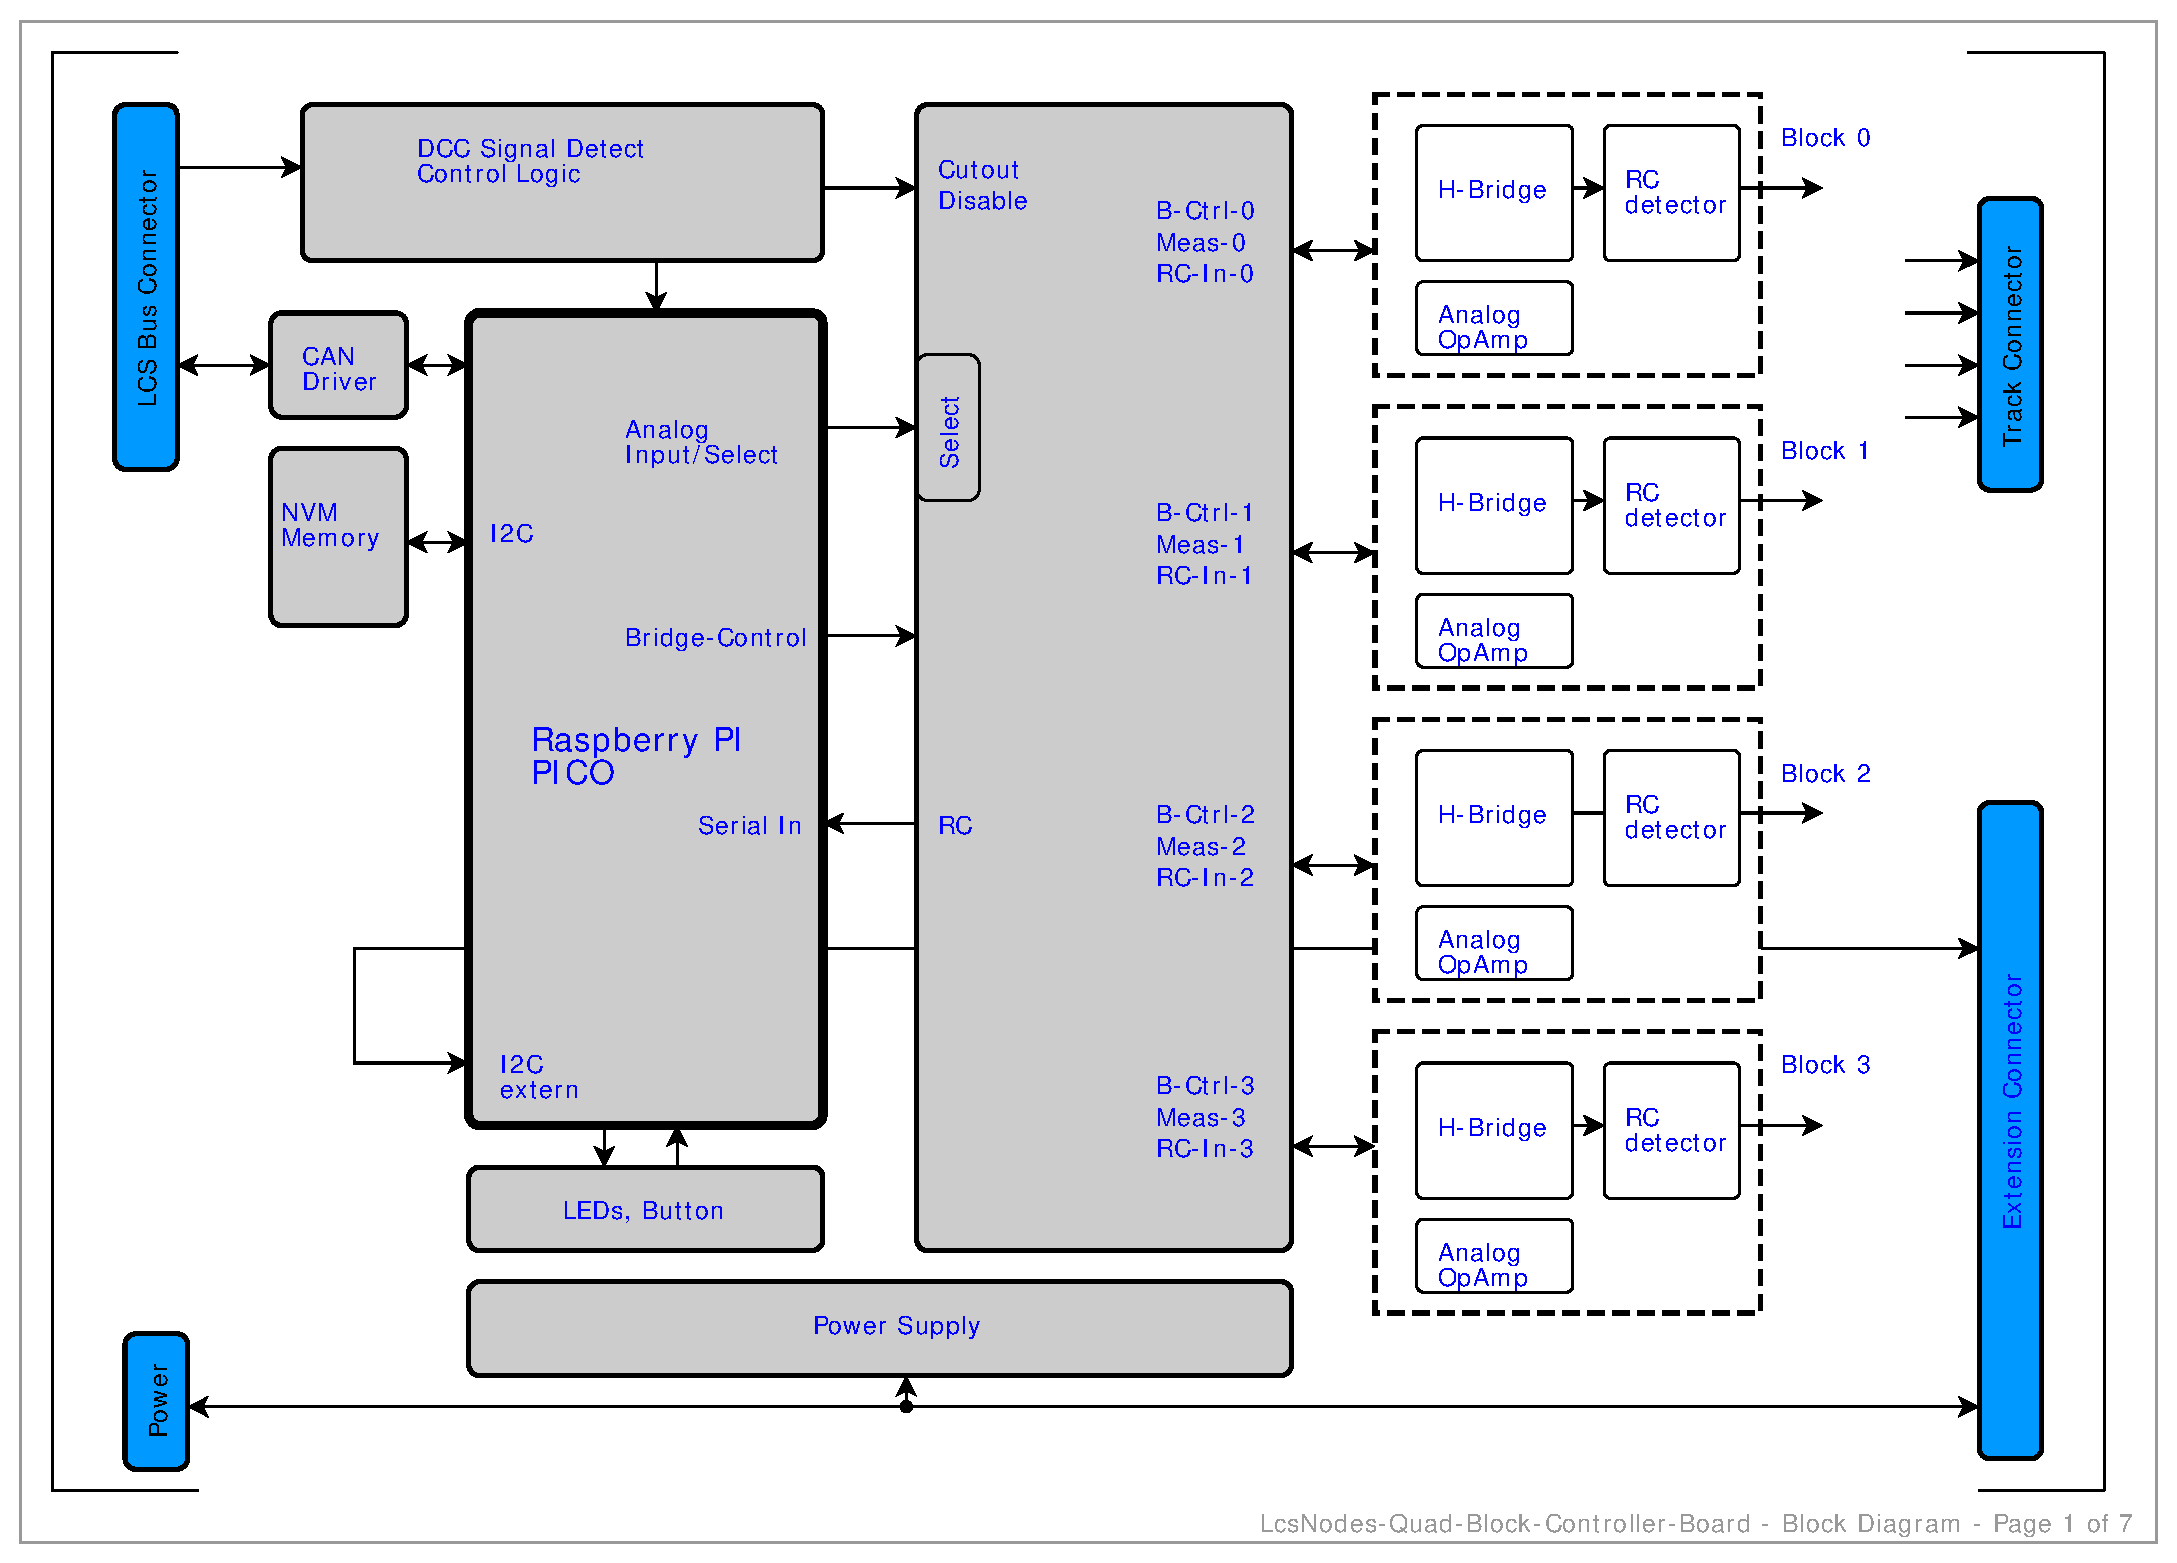
\includegraphics[page=1, width=0.9\textwidth]{./Schematics/Schematic_LcsNodes-Quad-Block-Controller.pdf}
    %\label{fig:schematic}
\end{figure}
\FloatBarrier

\subsection{Main Controller}

The first schematic shows the main controller Raspberry PI Pico, the level shifters required for the extension connector pins, the CAN bus driver and the non-volatile memory. This part is very similar to the main controller board shown in the previous chapters.

\begin{figure}[htbp]
    \centering
    \includegraphics[page=2, width=0.9\textwidth]{./Schematics/Schematic_LcsNodes-Quad-Block-Controller.pdf}
    %\label{fig:schematic}
\end{figure}
\FloatBarrier

\subsection{DCC Signal Input}

The next schematic shows the DCC signal receiver for the DCC signal coming from the base station. The block controller will take the DCC signal and eventually feed it to the H-Bridge power module. The DCC signal itself is also the mechanism to synchronize other signals such as the PWM signal generated locally on the block controller board. Since the DCC signal lines are decoupled from the rest of the logic via an OptoCoupler, all that we receive via the incoming signals are a zero state, i.e both lines are short circuited already or simply not powered, or in "+" or "-" signal state. Note that we cannot distinguish between a cutout signal and no power on the signal lines. The enabling and disabling of the power module needs to come from dedicated LCS messages to the node and cannot be derived from the DCC signal lines.

\begin{figure}[htbp]
    \centering
    \includegraphics[page=6, width=0.9\textwidth]{./Schematics/Schematic_LcsNodes-Quad-Block-Controller.pdf}
    %\label{fig:schematic}
\end{figure}
\FloatBarrier

In addition to recognizing the DCC cutout situation, we need to worry about several block controllers receiving that signal. Not all will switch into cutout mode at exactly the same time. This could potentially become a short circuit problem if block N is still powered, and block N + 1 already in cutout mode. A locomotive crossing from a still powered track to an already short circuited track will short circuit the powered track. To address this issue, the signal detector will generate a short window of about four microseconds where the power module input signal is put in the "high impedance" state when detecting a change into the short circuit state. And likewise, at the end of the cutout, there is the same window before leaving the cutout state. For PWM signals, the active part of the duty cycle drives the H-bridge to either a positive or negative output, the passive part will put the bridge into high-impedance.

\subsection{H-Bridge Decoding Logic}

There are four command to control the H-bridge. All decoding logic for the power unit control is done with dual 4-1 selectors. The signal from the opto-coupler is actually inverted, the wires need to be crossed for DCC signal input. All other signals are active high signals. 

\begin{figure}[htbp]
    \centering
    \includegraphics[page=3, width=0.9\textwidth]{./Schematics/Schematic_LcsNodes-Quad-Block-Controller.pdf}
    %\label{fig:schematic}
\end{figure}
\FloatBarrier

The bridge overall state, i.e. whether active or disconnected is controlled by an OR/AND gate, which will disable the bridge when both control signals are zero. For PWM mode, one side of the bridge will be at the zero level while the other will be the PWM signal. The PWM mode output of the bridge will thus be either a voltage for the "high" phase or disconnected for the "low" phase of the PWM signal.

The quad controller is pushing the Raspberry Pi Pico to its limits form a pin perspective. One could argue that the controller itself could just emits the correct control signals to the H-Bridge. True, but there are just not enough pins. Another argument for the decoding logic is that other H-Bridges can one day be used without changing the firmware to control them. 

\subsection{Power Unit}

Next is the power unit. The workings have already been described in the chapter on power units. The power unit is a H-Bridge with a current consumption measurement. The analog voltage across the shunt resistor is amplified and read in by the controller. Four H-Bridges need four analog inputs on the controller which we don't have on the Raspberry Pi PICO. All analog input signals are therefore multiplexed to one analog input port. We can thus read only one current measurement at a time.

\begin{figure}[htbp]
    \centering
    \includegraphics[page=4, width=0.9\textwidth]{./Schematics/Schematic_LcsNodes-Quad-Block-Controller.pdf}
    %\label{fig:schematic}
\end{figure}
\FloatBarrier

\subsection{Railcom Support}

For DCC Railcom support, the schematic shown below is the RailCom signal detector part. As explained in the DCC chapter, when Railcom is enabled, the decoders will put Railcom datagrams onto the track, which are detected by the circuitry shown below. The controller will just read in the serial communication and decode the datagrams. Although the component is optional, it should be on the board in any case, just to be flexible.

\begin{figure}[htbp]
    \centering
    \includegraphics[page=5, width=0.9\textwidth]{./Schematics/Schematic_LcsNodes-Quad-Block-Controller.pdf}
    %\label{fig:schematic}
\end{figure}
\FloatBarrier

\subsection{Power Supply and Connector}

And last but not least, there is a power supply and the connectors for the quad block controller board.

\begin{figure}[htbp]
    \centering
    \includegraphics[page=7, width=0.9\textwidth]{./Schematics/Schematic_LcsNodes-Quad-Block-Controller.pdf}
    %\label{fig:schematic}
\end{figure}
\FloatBarrier

\subsection{Quad Block Controller PCB}

The quad controller is implemented on a 10x16cm board layout. As you can see, it is a dense board. Even the place below the PICO board is used. Without SMD parts, this board would for sure not fit onto a 10x16Cm layout.

\begin{tikzpicture}[scale=0.9, transform shape]

    \draw[help lines, gray!50, dashed] (0,0) grid( 16,8);
    \node at (8,4) {picture};

\end{tikzpicture}


Well, that is the quad block controller. It is so to speak a maximum configuration. When designing a block controller with just two blocks, just take out one H-Bridge mode decoder and one Railcom detector. Furthermore, the L6205 dual H-Bridge can be configured to deliver twice the amperage. For larger scales a version of the block controller needs to be available that delivers on two blocks 5.6 Amps. There could also be a board that just has one block, which would be a classical booster. There could also be a board that has a power H-Bridge piggybacked on top, and so on. This chapter showed a full fledged four channel version, other combinations would still rest on the same core building blocks described.


\section{Dual Block Controller}

For some use cases, a quad controller is perhaps a bit too much. How about a block controller with just two channels. And in addition to running two blocks each how about a mono board with one higher amperage output. A nice feature of the L6205 dual bridge chip is that it allows to connect the two bridges in parallel delivering 5.6 instead of two times 2.8 Ampere. Let's design such a dual block controller board. Setting jumpers on the board will configure a mono block controller with 5.6 Amps or a dial block controller with two times 2.8 Amps. This way we also have a nice booster unit for larger scales. The overall design of the combo block controller design follows the building blocks outlined before. Here is the block diagram.

\subsection{Block Diagram}

\begin{figure}[htbp]
    \centering
    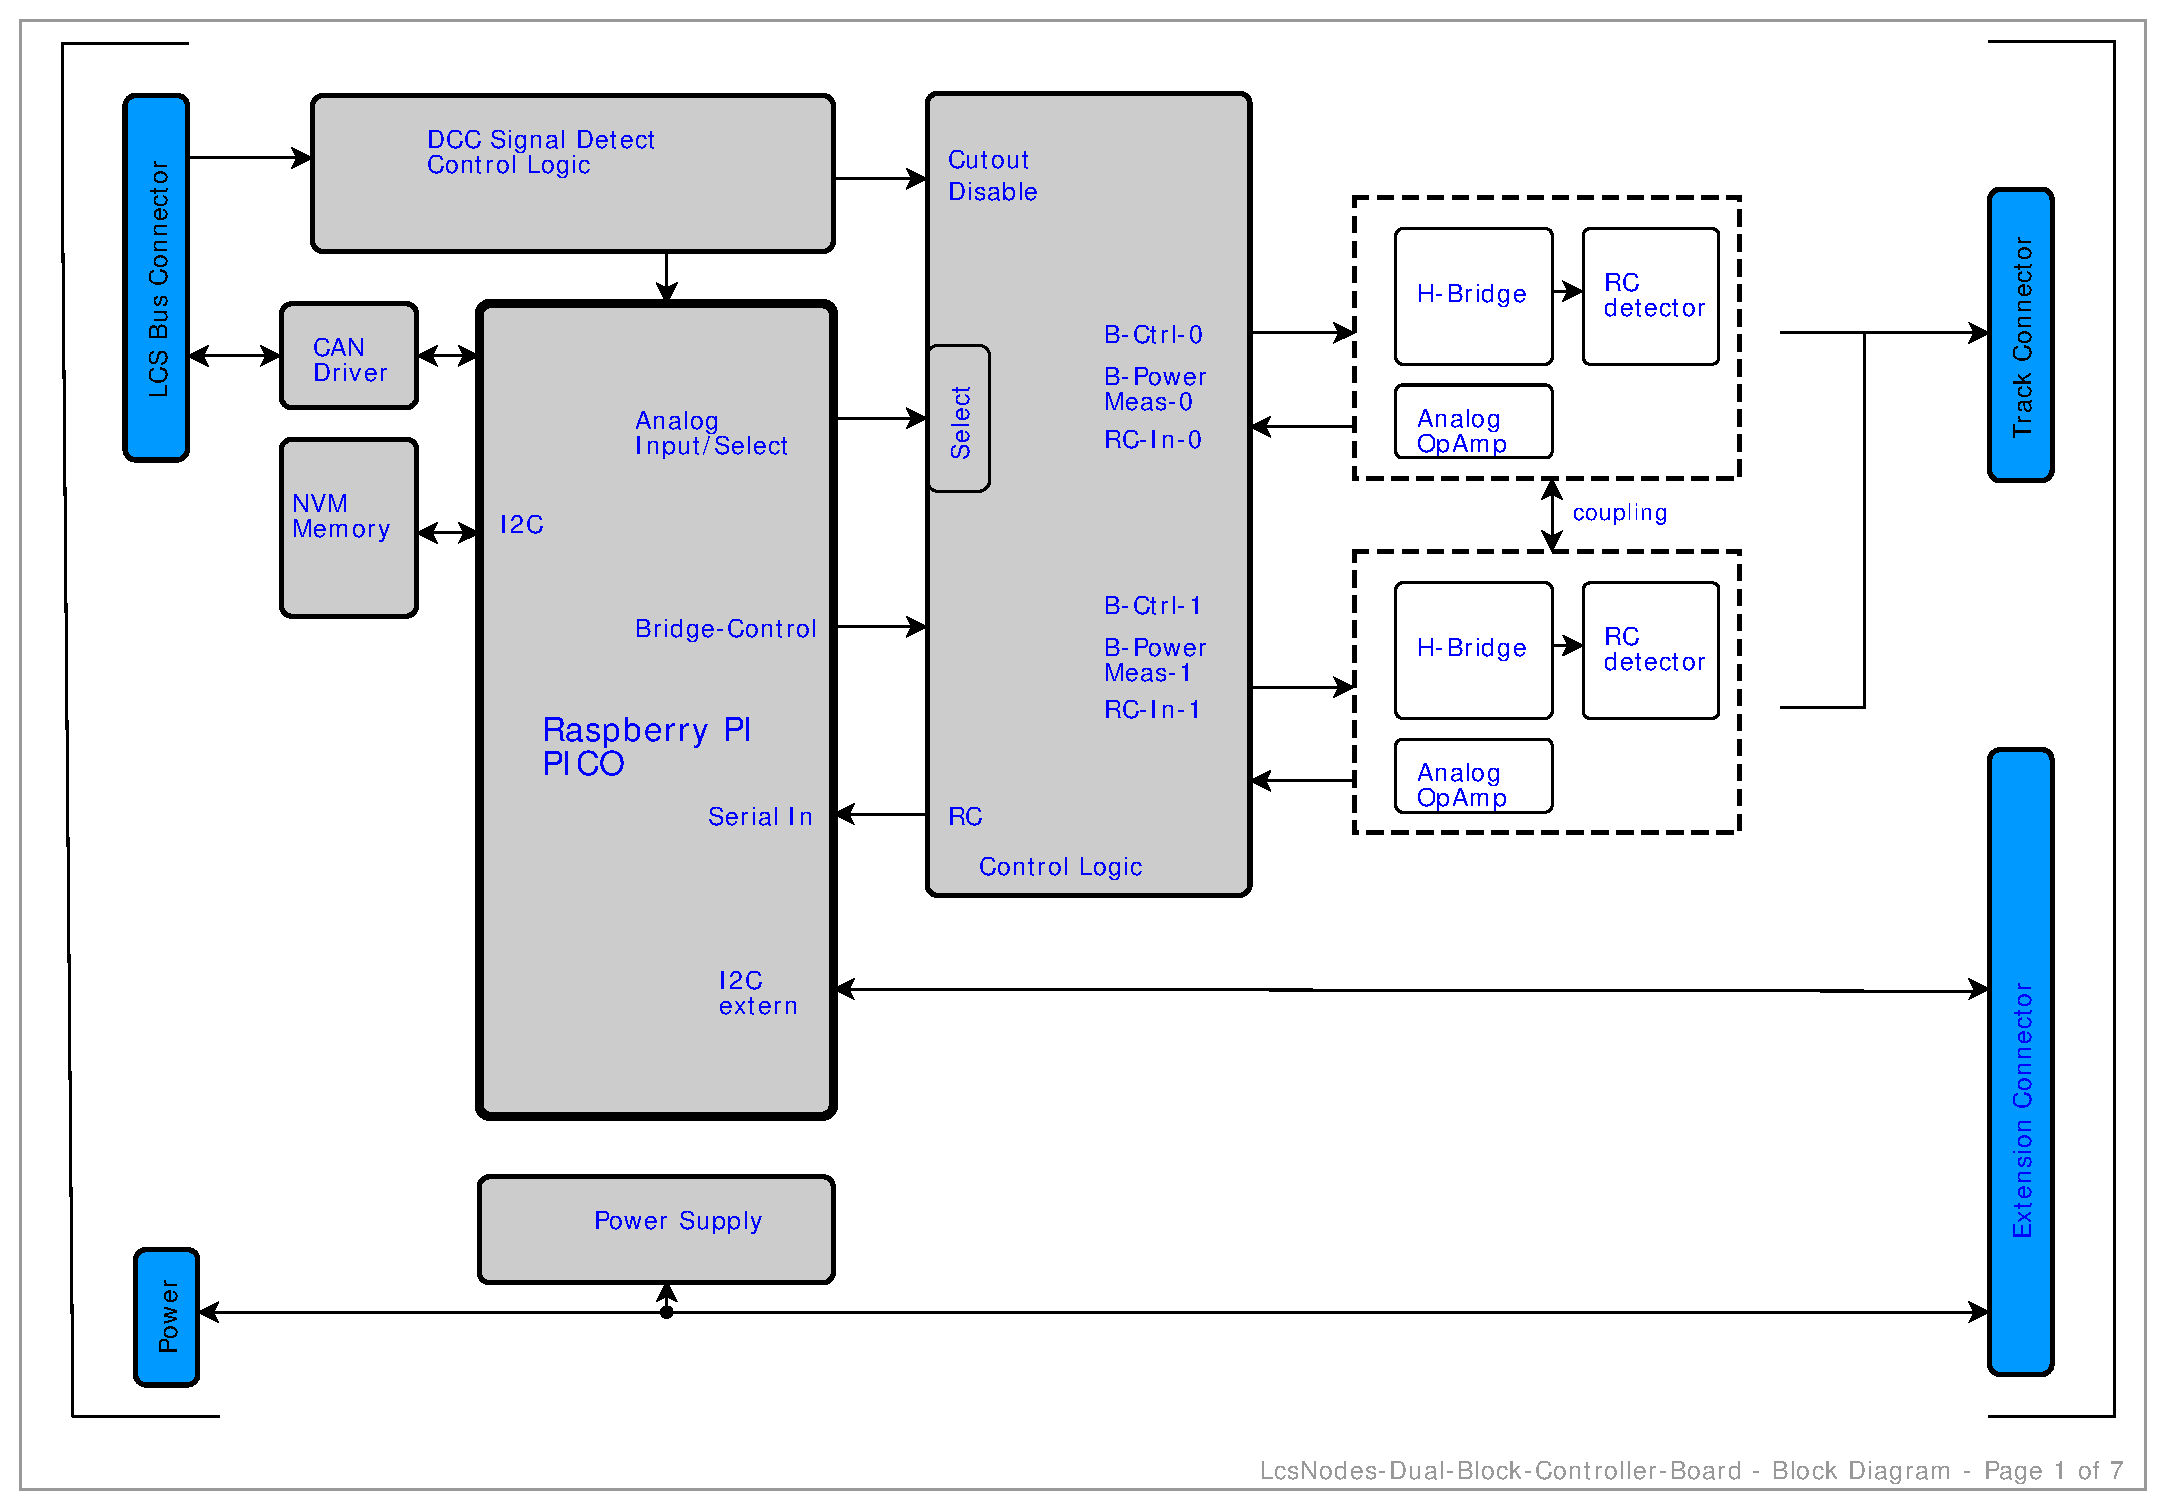
\includegraphics[page=1, width=0.9\textwidth]{./Schematics/Schematic_LcsNodes-Dual-Block-Controller.pdf}
    %\label{fig:schematic}
\end{figure}
\FloatBarrier

\subsection{Main Controller}

The main controller and the DCC signal decoding logic are identical to the quad controller.

\begin{figure}[htbp]
    \centering
    \includegraphics[page=2, width=0.9\textwidth]{./Schematics/Schematic_LcsNodes-Dual-Block-Controller.pdf}
    %\label{fig:schematic}
\end{figure}
\FloatBarrier


\subsection{DCC Signal Input}

\begin{figure}[htbp]
    \centering
    \includegraphics[page=3, width=0.9\textwidth]{./Schematics/Schematic_LcsNodes-Dual-Block-Controller.pdf}
    %\label{fig:schematic}
\end{figure}
\FloatBarrier

\subsection{H-Bridge decoding logic}

The Dual H-Bridge control logic implements the same logic, however since there are only two channels, the enable logic is implemented slightly different. There is also a set of jumpers that will put the two H-Bridges in parallel mode. When the H-bridge is configured to run in that mode, the outputs are connected in parallel. The control logic is that of channel zero.

\begin{figure}[htbp]
    \centering
    \includegraphics[page=4, width=0.9\textwidth]{./Schematics/Schematic_LcsNodes-Dual-Block-Controller.pdf}
    %\label{fig:schematic}
\end{figure}
\FloatBarrier

\subsection{Dual Power Unit}

The rest of the schematic is straightforward and other than we only need two instead of four units of RailCom, current amplifier and connectors is largely identical. Since we only have two current measurement units, there is no need to multiplex the analog signal. 

\begin{figure}[htbp]
    \centering
    \includegraphics[page=5, width=0.9\textwidth]{./Schematics/Schematic_LcsNodes-Dual-Block-Controller.pdf}
    %\label{fig:schematic}
\end{figure}
\FloatBarrier

\subsection{Dual RailCom Detect}

\begin{figure}[htbp]
    \centering
    \includegraphics[page=6, width=0.9\textwidth]{./Schematics/Schematic_LcsNodes-Dual-Block-Controller.pdf}
    %\label{fig:schematic}
\end{figure}
\FloatBarrier

\subsection{Connector and Power Supply}

\begin{figure}[htbp]
    \centering
    \includegraphics[page=7, width=0.9\textwidth]{./Schematics/Schematic_LcsNodes-Dual-Block-Controller.pdf}
    %\label{fig:schematic}
\end{figure}
\FloatBarrier

\subsection{Dual Block Controller PCB}

The dual controller is implemented on a 10x12cm board layout. As you can see, it is a dense board. Even the place below the PICO board is used. Without SMD parts, this board would for sure not fit onto a 10x12Cm layout.

\begin{tikzpicture}[scale=0.9, transform shape]

    \draw[help lines, gray!50, dashed] (0,0) grid( 16,8);
    \node at (8,4) {picture};

\end{tikzpicture}

\subsection{Block Controller Firmeware}


... wrap it up ...

... firmware comes after the extension board chapters ...


\section{H-Bridge control revised}

When looking at the overall schematics, a lot of discrete logic is required to control the H-Bridges. This is largely to the fact that the analog and digital world are supported by the block controller. Furthermore, as far as the quad controller goes, we simply run out of pins of the main controller platform and need a little help through decoding control signals outside of the controller chip.

What if we can use other features inside the controller chip for this decoding work ? When looking at the Raspberry Pi PICO controller the PIO state machine is a highly versatile output controller. Almost a processor in itself. As already mentioned, the the CAN bus interface is already implemented as a PIO program instead of the typical CAN bus controller peripheral. How about using the PIO state machines also for our H-Bridge control. 

Consider that we can redefine the H-Bridge control signals slightly. The H-Bridge enable line is derived from the two  input control lines, using the unassigned state of 0b11 as putting the H-Bridge into disconnected mode. All it needs is a simple NAND gate. Control input 0b00 still puts the bridge into short circuit for the DCC cutout feature, 0b01 and 0b10 are still the PWM mode options. 

Instead of routing the DCC signals to the multiplexers, they are routed to two input pins on the PICO. The PIO program uses them as input to detect the cutout period and also to pass on the DCC signal. Since a PIO program is a program, we can also just implement the quiet period at the beginning of the cutout period. In other words, the entire logic of DCC signal input and H-Bridge control moves into the PICO. 

This is future work.... stay tuned.

\section{Summary}

This chapter presented the block controllers. Although rather simple in the individual building blocks, it was a champions league effort when it came to the PCB board design. The quad controller is the most complex board of all the board described in this book so far. The dual block controller shows that with little effort and the right H-Bridge chip, a mono block controller with twice the amperage and a dual block controller can nicely be combined. We also abstracted the control of the power unit. From a firmware perspective, the bridge is controlled with two bits, putting the bridge in disconnected mode, PWM modes forward and reverse and finally DCC mode.

